\section{Ablation, Attribution and Search-Time Tables}
\label{app:v2results}

Tables labelled search-time use each method's own selection split during the search; they are not held-out and are not comparable across methods. Tables without final-set columns are marked pending.

\begin{table}[t]
\centering
\scriptsize
\setlength{\tabcolsep}{3.5pt}
\caption{Stock-gate and rule-P hill-climb at the same rollout count, with per-seed paired deltas to the seed in points and promotion counts (means per search). Descriptive and exploratory: no tests. The best-of-$k$ row draws $k$ independent one-shot proposals per seed on Suite C and keeps the best on the optimization set. It is truncated at $k=6/6/8$ proposals (140/140/180 counted rollouts) for seeds 0/1/2, paused to fund the Suite B stock-gate arm, and is exploratory and descriptive only. (placeholder)}
\label{tab:e12}
\begin{tabular}{lcccccc}
\toprule
Arm & Seed 0 & Seed 1 & Seed 2 & Screened & Promoted & Returned = seed \\
\midrule
\multicolumn{7}{l}{\textit{Suite A}} \\
Rule P & \pend{+0.0} & \pend{+8.1} & \pend{+0.0} & \pend{8.7} & \pend{1.0} & \pend{2 of 3} \\
Stock gate & \pend{+7.4} & \pend{+5.2} & \pend{+6.1} & \pend{8.3} & \pend{6.0} & \pend{0 of 3} \\
\midrule
\multicolumn{7}{l}{\textit{Suite C}} \\
Rule P & \pend{+3.5} & \pend{+2.2} & \pend{+6.7} & \pend{10.3} & \pend{2.3} & \pend{0 of 3} \\
Stock gate & \pend{+4.8} & \pend{+4.6} & \pend{+4.9} & \pend{10.0} & \pend{3.0} & \pend{0 of 3} \\
Best of $k$ & \pend{+3.0} & \pend{+4.7} & \pend{+3.1} & -- & -- & -- \\
\bottomrule
\end{tabular}
\end{table}

\begin{table*}[t]
\centering
\scriptsize
\setlength{\tabcolsep}{3.5pt}
\caption{Suite D ablation cells on the 40 test tasks scored five times each; the 65 held-out tasks (selection and test) are descriptive. All cells are hill-climb with the stock gate except where the gate or the history is the factor. Each cell changes one factor against the PT reference. The Holm family has 11 contrasts. Differences below the pre-registered equivalence margin of 10 points are written inconclusive, not equal. (placeholder)}
\label{tab:ablation}
\begin{tabular}{lcccccrr}
\toprule
Cell & Seeds & $\Delta$ vs seed [CI] & $p_{\mathrm{Holm}}$ vs seed & $\Delta$ vs PT [CI] & $p_{\mathrm{Holm}}$ vs PT & Promoted per search & Returned = seed \\
\midrule
One-shot control & 3 & \pend{+6.3 [$-$5.1, +17.7]} & -- & \pend{$-$0.8 [$-$14.8, +13.2]} & \pend{1.000} & \pend{1.7} & \pend{0 of 3} \\
Prompt only (P) & 3 & \pend{+4.6 [$-$6.0, +15.2]} & \pend{1.000} & \pend{$-$2.5 [$-$16.5, +11.5]} & \pend{1.000} & \pend{5.0} & \pend{0 of 3} \\
Tools only (T) & 3 & \pend{+2.6 [$-$8.2, +13.4]} & \pend{1.000} & \pend{$-$4.5 [$-$18.5, +9.5]} & \pend{1.000} & \pend{4.0} & \pend{0 of 3} \\
Prompt and tools (PT), reference & 3 & \pend{+7.1 [$-$4.6, +18.8]} & \pend{1.000} & ref. & -- & \pend{4.3} & \pend{0 of 3} \\
PT with rule P & 3 & \pend{+7.4 [$-$3.7, +18.5]} & -- & \pend{+0.3 [$-$13.7, +14.3]} & \pend{1.000} & \pend{1.3} & \pend{0 of 3} \\
PT with one-stage gate & 3 & \pend{+2.3 [$-$8.3, +12.9]} & -- & \pend{$-$4.8 [$-$18.8, +9.2]} & \pend{1.000} & \pend{4.3} & \pend{0 of 3} \\
GEPA, prompt only & 3 & \pend{+5.8 [$-$5.5, +17.1]} & -- & \pend{$-$1.3 [$-$15.3, +12.7]} & \pend{1.000} & \pend{2.7} & \pend{0 of 3} \\
PT without fixed/broke history & 3 & \pend{+5.1 [$-$7.1, +17.3]} & -- & \pend{$-$2.0 [$-$16.0, +12.0]} & \pend{1.000} & \pend{4.3} & \pend{0 of 3} \\
\midrule
\multicolumn{8}{l}{Interaction PT $-$ P $-$ T (descriptive): \pend{$-$0.1 [$-$21.7, +21.5]}. P versus T: \pend{+2.0} points, $p_{\mathrm{Holm}}$ \pend{1.000}.} \\
\bottomrule
\end{tabular}
\end{table*}

\begin{table}[t]
\centering
\scriptsize
\setlength{\tabcolsep}{3.5pt}
\caption{Decomposition of Suite D champions that edit both surfaces: paired delta of the whole artifact, of its prompt edits on the seed tools, and of its tool edits on the seed prompt, in points. A gap near zero means the parts add up. (placeholder)}
\label{tab:decomp}
\begin{tabular}{lrrrr}
\toprule
Champion & Whole artifact & Prompt part & Tool part & Whole minus parts \\
\midrule
pt seed 0 & \pend{$-$1.2} & \pend{$-$0.4} & \pend{$-$1.8} & \pend{+1.0} \\
pt seed 1 & \pend{+5.5} & \pend{+3.5} & \pend{+3.8} & \pend{$-$1.8} \\
pt seed 2 & \pend{+10.3} & \pend{+7.3} & \pend{+3.4} & \pend{$-$0.5} \\
rulep seed 0 & \pend{+3.6} & \pend{+2.2} & \pend{+1.9} & \pend{$-$0.4} \\
onestage seed 1 & \pend{+6.5} & \pend{+5.2} & \pend{+3.6} & \pend{$-$2.2} \\
onestage seed 2 & \pend{+5.1} & \pend{+2.1} & \pend{+1.4} & \pend{+1.6} \\
ctl seed 0 & \pend{+5.9} & \pend{+3.6} & \pend{+4.1} & \pend{$-$1.9} \\
pt seed 1 & \pend{+4.3} & \pend{+0.9} & \pend{+2.8} & \pend{+0.6} \\
\bottomrule
\end{tabular}
\end{table}

\begin{table*}[t]
\centering
\scriptsize
\setlength{\tabcolsep}{3.5pt}
\caption{Cost, regressions and selection-to-final shrinkage per arm. USD per point is optimizer cost per seed divided by the final-set gain in points. Pass to fail counts tasks the seed solved and the champion fails, per seed. Shrinkage is selection gain minus final gain, in points, and is zero for a seed that returned the seed artifact. (placeholder)}
\label{tab:rq4}
\begin{tabular}{lrrrrrr}
\toprule
Arm & USD per point & Pass to fail & Protect-set violations & Selection gain & Final gain & Shrinkage \\
\midrule
\multicolumn{7}{l}{\textit{Suite A, SpreadsheetBench verified-400 (Gemma-4-31B-it)}} \\
\midrule
Meta-Harness & \pend{18.7} & \pend{3.1} & \pend{2.5} & \pend{+5.7} & \pend{$-$1.1} & \pend{+6.8} \\
GEPA & \pend{0.8} & \pend{1.4} & \pend{1.6} & \pend{+12.3} & \pend{+3.2} & \pend{+9.1} \\
EvoSkill & \pend{1.5} & \pend{2.7} & \pend{1.7} & \pend{+11.2} & \pend{+3.6} & \pend{+7.6} \\
WikiSkill (community) & \pend{0.4} & \pend{2.4} & \pend{3.2} & \pend{+13.7} & \pend{+5.3} & \pend{+8.4} \\
MIPROv2 & \pend{0.7} & \pend{0.0} & \pend{2.2} & \pend{+15.1} & \pend{+5.3} & \pend{+9.8} \\
Trace2Skill & \pend{1.1} & \pend{3.0} & \pend{1.4} & \pend{+8.8} & \pend{+5.5} & \pend{+3.3} \\
ACE & \pend{1.0} & \pend{4.6} & \pend{1.1} & \pend{+10.2} & \pend{+5.6} & \pend{+4.6} \\
SkillOpt & \pend{0.6} & \pend{0.0} & \pend{2.2} & \pend{+11.3} & \pend{+6.0} & \pend{+5.4} \\
CapEvolve as shipped, stock gate$^{\S}$ & \pend{2.8} & \pend{1.6} & \pend{1.9} & \pend{+6.3} & \pend{+4.4} & \pend{+1.9} \\
CapEvolve HC, rule P & \pend{2.9} & \pend{4.6} & \pend{1.5} & \pend{+7.7} & \pend{+3.2} & \pend{+4.5} \\
CapEvolve AO, rule P & \pend{2.9} & \pend{3.4} & \pend{2.4} & \pend{+5.6} & \pend{+4.1} & \pend{+1.5} \\
\midrule
\multicolumn{7}{l}{\textit{Suite B, $\tau^2$ retail, sealed test-40 (gpt-oss-120b)}} \\
\midrule
HarnessLens & \pend{9.6} & \pend{3.8} & \pend{1.1} & \pend{+2.2} & \pend{$-$1.9} & \pend{+4.1} \\
GEPA & \pend{3.9} & \pend{0.1} & \pend{2.3} & \pend{+7.7} & \pend{+1.3} & \pend{+6.5} \\
CapEvolve HC, rule P & \pend{1.9} & \pend{3.9} & \pend{1.3} & \pend{+8.8} & \pend{+5.7} & \pend{+3.1} \\
CapEvolve AO, rule P & \pend{4.2} & \pend{1.6} & \pend{2.4} & \pend{+10.1} & \pend{+3.5} & \pend{+6.6} \\
\midrule
\multicolumn{7}{l}{\textit{Suite C, $\tau^2$ airline, official test-20 (development-exposed)}} \\
\midrule
GEPA & \pend{1.3} & \pend{2.1} & \pend{1.4} & \pend{+7.6} & \pend{+3.7} & \pend{+3.9} \\
HarnessLens & \pend{0.7} & \pend{3.8} & \pend{2.0} & \pend{+6.8} & \pend{+6.0} & \pend{+0.8} \\
CapEvolve as shipped, stock gate$^{\S}$ & \pend{0.7} & \pend{3.1} & \pend{2.2} & \pend{+7.4} & \pend{+7.4} & \pend{+0.0} \\
CapEvolve HC, rule P & \pend{4.8} & \pend{4.4} & \pend{1.3} & \pend{+7.2} & \pend{+2.6} & \pend{+4.5} \\
CapEvolve AO, rule P & \pend{5.4} & \pend{2.5} & \pend{1.5} & \pend{+5.8} & \pend{+1.6} & \pend{+4.1} \\
\bottomrule
\end{tabular}
\end{table*}

\begin{table*}[t]
\centering
\scriptsize
\caption{Failure types of the seed artifact's failed tasks, summed over seeds and trials-pooled tasks. Search-time, failed seed tasks on each run's selection split; deterministic labels from scorer feedback, no model judge, not held-out. Forgotten rule or step: a required write was never called ($\tau^2$). Tool misuse: a write with wrong arguments. Output/contract: no output file (Suite A) or unmet communication assertion ($\tau^2$). Knowledge or rule gap: an output file exists and fails the checks (Suite A).}
\label{tab:attrib-failure-types}
\resizebox{\textwidth}{!}{%
\begin{tabular}{@{}llrrrrrrrr@{}}
\toprule
Suite & Arm & Failed & forgotten rule or step & tool misuse & unexpected side effect & output / contract & knowledge or rule gap & infra (unscorable) & other \\
\midrule
A & CapEvolve AO, rule P & 59 & 0 & 0 & 0 & 26 & 28 & 5 & 0 \\
A & CapEvolve HC, rule P & 54 & 0 & 0 & 0 & 27 & 21 & 6 & 0 \\
A & CapEvolve, stock gate & 57 & 0 & 0 & 0 & 26 & 26 & 5 & 0 \\
B & CapEvolve AO, rule P & 58 & 18 & 24 & 5 & 5 & 0 & 1 & 5 \\
B & CapEvolve HC, rule P & 63 & 23 & 25 & 4 & 3 & 0 & 1 & 7 \\
B & One-shot control & 60 & 17 & 27 & 4 & 5 & 0 & 1 & 6 \\
C & CapEvolve AO, rule P & 29 & 10 & 11 & 5 & 0 & 0 & 0 & 3 \\
C & CapEvolve HC, rule P & 31 & 12 & 13 & 1 & 2 & 0 & 0 & 3 \\
C & CapEvolve, stock gate & 28 & 9 & 12 & 1 & 2 & 0 & 1 & 3 \\
C & One-shot control & 29 & 10 & 11 & 0 & 0 & 0 & 1 & 7 \\
D & D: control (CTL) & 58 & 16 & 23 & 3 & 5 & 0 & 1 & 10 \\
D & D: CapEvolve P & 64 & 22 & 19 & 3 & 6 & 0 & 2 & 12 \\
D & D: CapEvolve P+T & 68 & 28 & 22 & 3 & 5 & 0 & 0 & 10 \\
D & D: CapEvolve T & 62 & 24 & 23 & 5 & 4 & 0 & 0 & 6 \\
D & D: one-stage gate & 67 & 23 & 24 & 2 & 10 & 0 & 2 & 6 \\
D & D: Rule P & 67 & 22 & 25 & 4 & 4 & 0 & 1 & 11 \\
D & D: no history & 61 & 20 & 25 & 2 & 7 & 0 & 0 & 7 \\
\bottomrule
\end{tabular}
}
\end{table*}

\begin{table*}[t]
\centering
\scriptsize
\caption{Promotions per search and inert searches (the returned artifact equals the seed), per arm. Search-time, each method's own selection split, not held-out. Counts are for the state of each search at the time of the run (still running = searches not yet finished, so inert counts can still change). Promotion definitions differ by method (accepted by the method's own rule) and are not comparable across methods.}
\label{tab:attrib-promotions}
\begin{tabular}{@{}llrrrrrrr@{}}
\toprule
Suite & Arm & Searches & Cands & Promotions & Per search & Inert & Running & Crashed \\
\midrule
A & GEPA & 3 & 40 & 23 & 7.67 & 0 & 3 & 0 \\
A & SkillOpt & 3 & 18 & 11 & 3.67 & 0 & 3 & 0 \\
A & Meta-Harness & 3 & 24 & 10 & 3.33 & 0 & 1 & 0 \\
A & EvoSkill & 3 & 18 & 17 & 5.67 & 0 & 2 & 0 \\
A & WikiSkill-comm. & 3 & 3 & 2 & 0.67 & 1 & 3 & 0 \\
A & Trace2Skill & 3 & 6 & 3 & 1.00 & 0 & 0 & 0 \\
A & ACE & 3 & 0 & 0 & 0.00 & 0 & 3 & 0 \\
A & MIPROv2 & 3 & 20 & 0 & 0.00 & 3 & 3 & 0 \\
A & CapEvolve HC & 3 & 8 & 1 & 0.33 & 2 & 3 & 0 \\
A & CapEvolve AO & 3 & 3 & 0 & 0.00 & 3 & 3 & 0 \\
A-E12 & CapEvolve HC, stock gate & 3 & 19 & 6 & 2.00 & 0 & 3 & 0 \\
B & One-shot control & 3 & 3 & 1 & 0.33 & 2 & 0 & 0 \\
B & GEPA & 3 & 43 & 16 & 5.33 & 0 & 3 & 0 \\
B & HarnessLens & 3 & 0 & 0 & 0.00 & 0 & 1 & 0 \\
B & CapEvolve HC & 3 & 9 & 0 & 0.00 & 3 & 3 & 0 \\
B & CapEvolve AO & 3 & 3 & 0 & 0.00 & 3 & 1 & 0 \\
C & One-shot control & 3 & 3 & 1 & 0.33 & 2 & 0 & 0 \\
C & GEPA & 3 & 27 & 12 & 4.00 & 0 & 3 & 0 \\
C & CapEvolve HC & 3 & 9 & 0 & 0.00 & 3 & 3 & 0 \\
C & CapEvolve AO & 3 & 1 & 0 & 0.00 & 3 & 0 & 0 \\
C-E12 & CapEvolve HC, stock gate & 3 & 16 & 3 & 1.00 & 1 & 3 & 0 \\
C-E12 & Best-of-$k$ & 3 & 15 & 0 & 0.00 & 0 & 3 & 0 \\
\bottomrule
\end{tabular}
\end{table*}

\begin{table*}[t]
\centering
\scriptsize
\caption{Regressions per promotion and net gain for CapEvolve searches. Search-time, own selection split of each run, not held-out. Fixed and broke: tasks moving across the pass line (reward 0.5) relative to the parent. Protect viol.: seed-solid tasks that score below 1 at the candidate. Fresh $\Delta$: promoted candidate minus its baseline on fresh confirmation trials (Rule P only), the least biased within-search gain. Rejected: mean tasks broken by rejected candidates (candidates still pending are excluded).}
\label{tab:attrib-regression}
\begin{tabular}{@{}llrrrrrrrr@{}}
\toprule
Suite & Arm & Cands & Promoted & Fixed/prom. & Broke/prom. & Net/prom. & Broke/rej. & Protect viol./prom. & Fresh $\Delta$/prom. \\
\midrule
A & CapEvolve HC & 5 & 1 & 7.0 & 3.0 & 4.0 & 5.0 & 3.0 & 0.133 \\
A & CapEvolve HC, stock gate & 16 & 6 & 8.3 & 2.5 & 5.8 & 3.4 & 2.2 & -- \\
B & CapEvolve HC & 10 & 0 & -- & -- & -- & 7.2 & -- & -- \\
B & One-shot control & 3 & 1 & 11.0 & 4.0 & 7.0 & 8.0 & 4.0 & -- \\
C & CapEvolve HC & 12 & 0 & -- & -- & -- & 2.0 & -- & -- \\
C & CapEvolve HC, stock gate & 16 & 3 & 4.7 & 1.3 & 3.3 & 3.6 & 1.0 & -- \\
C & One-shot control & 3 & 1 & 5.0 & 1.0 & 4.0 & 2.5 & 1.0 & -- \\
\bottomrule
\end{tabular}
\end{table*}

\begin{table*}[t]
\centering
\scriptsize
\caption{Edit attribution by capability surface for CapEvolve candidates. Search-time, own selection split of each run (A: val-40, B: opt-49, C: opt-20), not held-out. Touching/total candidates, promoted among those touching, mean selection-split change vs parent, mean tasks fixed and broken (pass = reward $\ge$ 0.5), and Spearman correlation between lines changed on the surface and the change. n/a: surface touched by all or none, so no contrast. Selection-split changes are optimistic and noisy.}
\label{tab:attrib-surface}
\resizebox{\textwidth}{!}{%
\begin{tabular}{@{}llllrrrrr@{}}
\toprule
Suite & Arm & Surface & Touch & Promoted & $\Delta$ sel. & Fixed & Broke & $\rho$ \\
\midrule
A & CapEvolve HC, rule P & system\_prompt & 11/11 & 2 & 0.218 & 9.6 & 1.5 & 0.84 \\
A & CapEvolve HC, rule P & task\_template & 11/11 & 2 & 0.218 & 9.6 & 1.5 & 0.40 \\
A & CapEvolve, stock gate & system\_prompt & 36/36 & 7 & 0.017 & 3.6 & 2.9 & -0.53 \\
A & CapEvolve, stock gate & task\_template & 36/36 & 7 & 0.017 & 3.6 & 2.9 & -0.25 \\
B & CapEvolve HC, rule P & system\_prompt & 9/16 & 0 & 0.010 & 7.3 & 6.9 & 0.22 \\
B & CapEvolve HC, rule P & tool\_code & 14/16 & 0 & -0.007 & 6.8 & 7.1 & -0.16 \\
B & One-shot control & system\_prompt & 3/3 & 1 & 0.017 & 7.7 & 6.7 & n/a \\
B & One-shot control & tool\_code & 3/3 & 1 & 0.017 & 7.7 & 6.7 & n/a \\
C & CapEvolve HC, rule P & system\_prompt & 16/16 & 2 & 0.072 & 3.1 & 1.7 & 0.55 \\
C & CapEvolve HC, rule P & tool\_code & 16/16 & 2 & 0.072 & 3.1 & 1.7 & 0.61 \\
C & CapEvolve, stock gate & system\_prompt & 28/29 & 3 & -0.059 & 2.0 & 3.1 & -0.25 \\
C & CapEvolve, stock gate & tool\_code & 29/29 & 3 & -0.062 & 2.0 & 3.2 & -0.29 \\
C & One-shot control & system\_prompt & 3/3 & 1 & 0.088 & 3.7 & 2.0 & n/a \\
C & One-shot control & tool\_code & 3/3 & 1 & 0.088 & 3.7 & 2.0 & n/a \\
\bottomrule
\end{tabular}
}
\end{table*}

\begin{table*}[t]
\centering
\scriptsize
\caption{Surface by failure type: seed-failed tasks fixed by CapEvolve candidates, grouped by the candidate's dominant edited surface (most changed lines). Search-time, fixes counted on each run's selection split over all candidates, promoted ones in parentheses, not held-out. A task counts as fixed when it fails at the parent and passes at the candidate; the count includes noise flips and is not a measure of cause. Types not listed were not fixed.}
\label{tab:attrib-surface-failure}
\resizebox{\textwidth}{!}{%
\begin{tabular}{@{}llrrrrrrrrr@{}}
\toprule
Suite & Dominant surface & communication & infra & missing\_action & no\_output\_file & other & state\_side\_effect & was\_passing\_or\_unlabelled & wrong\_argument & wrong\_result \\
\midrule
A & system\_prompt & 0 (0) & 1 (1) & 0 (0) & 53 (23) & 0 (0) & 0 (0) & 20 (7) & 0 (0) & 44 (26) \\
B & tool\_code & 3 (1) & 0 (0) & 28 (3) & 0 (0) & 11 (1) & 3 (1) & 0 (0) & 37 (5) & 0 (0) \\
B & unavailable & 0 (0) & 0 (0) & 4 (0) & 0 (0) & 2 (0) & 0 (0) & 0 (0) & 3 (0) & 0 (0) \\
C & tool\_code & 4 (0) & 0 (0) & 31 (8) & 0 (0) & 7 (1) & 5 (0) & 5 (2) & 24 (8) & 0 (0) \\
C & unavailable & 2 (0) & 0 (0) & 4 (0) & 0 (0) & 0 (0) & 1 (0) & 0 (0) & 3 (0) & 0 (0) \\
\bottomrule
\end{tabular}}
\end{table*}

\begin{table*}[t]
\centering
\scriptsize
\caption{Selection-to-final shrinkage (selection-split gain minus final-set gain), per arm and seed. PENDING FINAL: the final-set column is empty until the final evaluation (cutoff 2026-10-13 06:00 UTC); the selection gain shown is search-time, on each method's own selection split, not held-out. Seeds that return the seed artifact have shrinkage 0 by construction (amendment 6).}
\label{tab:attrib-shrinkage}
\begin{tabular}{@{}llrrrrl@{}}
\toprule
Suite & Arm & Seed & Sel. gain & Final gain & Shrinkage & Inert \\
\midrule
A & CapEvolve HC, rule P & 0 & 0.171 & -- & -- & no \\
A & CapEvolve HC, rule P & 1 & 0.103 & -- & -- & no \\
A & CapEvolve HC, rule P & 2 & 0.000 & -- & -- & yes \\
A & CapEvolve AO, rule P & 0 & 0.000 & -- & -- & yes \\
A & CapEvolve AO, rule P & 1 & 0.000 & -- & -- & yes \\
A & CapEvolve AO, rule P & 2 & 0.000 & -- & -- & yes \\
A & GEPA & 0 & 0.325 & -- & -- & no \\
A & GEPA & 1 & 0.350 & -- & -- & no \\
A & GEPA & 2 & 0.375 & -- & -- & no \\
A & SkillOpt & 0 & 0.150 & -- & -- & no \\
A & SkillOpt & 1 & 0.300 & -- & -- & no \\
A & SkillOpt & 2 & 0.275 & -- & -- & no \\
A & Meta-Harness & 0 & 0.375 & -- & -- & no \\
A & Meta-Harness & 1 & 0.250 & -- & -- & no \\
A & Meta-Harness & 2 & 0.300 & -- & -- & no \\
A & EvoSkill & 0 & 0.250 & -- & -- & no \\
A & EvoSkill & 1 & 0.325 & -- & -- & no \\
A & EvoSkill & 2 & 0.300 & -- & -- & no \\
A & WikiSkill-comm. & 0 & 0.225 & -- & -- & no \\
A & WikiSkill-comm. & 1 & 0.300 & -- & -- & no \\
A & WikiSkill-comm. & 2 & 0.200 & -- & -- & no \\
A & Trace2Skill & 0 & 0.200 & -- & -- & no \\
A & Trace2Skill & 1 & 0.275 & -- & -- & no \\
A & Trace2Skill & 2 & 0.225 & -- & -- & no \\
A & ACE & 0 & 0.000 & -- & -- & yes \\
A & ACE & 1 & 0.000 & -- & -- & yes \\
A & ACE & 2 & -- & -- & -- & -- \\
A & MIPROv2 & 0 & 0.200 & -- & -- & no \\
A & MIPROv2 & 1 & 0.300 & -- & -- & no \\
A & MIPROv2 & 2 & 0.050 & -- & -- & no \\
B & CapEvolve HC, rule P & 0 & 0.000 & -- & -- & yes \\
B & CapEvolve HC, rule P & 1 & 0.000 & -- & -- & yes \\
B & CapEvolve HC, rule P & 2 & 0.000 & -- & -- & yes \\
B & CapEvolve AO, rule P & 0 & 0.000 & -- & -- & yes \\
B & CapEvolve AO, rule P & 1 & 0.000 & -- & -- & yes \\
B & CapEvolve AO, rule P & 2 & 0.000 & -- & -- & yes \\
B & GEPA & 0 & 0.160 & -- & -- & no \\
B & GEPA & 1 & 0.360 & -- & -- & no \\
B & GEPA & 2 & 0.120 & -- & -- & no \\
B & HarnessLens & 0 & -- & -- & -- & -- \\
B & HarnessLens & 1 & -- & -- & -- & -- \\
B & HarnessLens & 2 & -- & -- & -- & -- \\
B & One-shot control & 0 & 0.000 & -- & -- & yes \\
B & One-shot control & 1 & 0.143 & -- & -- & no \\
B & One-shot control & 2 & 0.000 & -- & -- & yes \\
C & CapEvolve HC, rule P & 0 & 0.150 & -- & -- & no \\
C & CapEvolve HC, rule P & 1 & 0.000 & -- & -- & yes \\
C & CapEvolve HC, rule P & 2 & 0.134 & -- & -- & no \\
C & CapEvolve AO, rule P & 0 & 0.000 & -- & -- & yes \\
C & CapEvolve AO, rule P & 1 & 0.000 & -- & -- & yes \\
C & CapEvolve AO, rule P & 2 & 0.000 & -- & -- & yes \\
C & GEPA & 0 & 0.200 & -- & -- & no \\
C & GEPA & 1 & 0.200 & -- & -- & no \\
C & GEPA & 2 & 0.100 & -- & -- & no \\
C & One-shot control & 0 & 0.237 & -- & -- & no \\
C & One-shot control & 1 & 0.000 & -- & -- & yes \\
C & One-shot control & 2 & 0.000 & -- & -- & yes \\
A-E12 & CapEvolve, stock gate & 0 & 0.286 & -- & -- & no \\
A-E12 & CapEvolve, stock gate & 1 & 0.349 & -- & -- & no \\
A-E12 & CapEvolve, stock gate & 2 & 0.322 & -- & -- & no \\
C-E12 & CapEvolve, stock gate & 0 & 0.237 & -- & -- & no \\
C-E12 & CapEvolve, stock gate & 1 & 0.000 & -- & -- & yes \\
C-E12 & CapEvolve, stock gate & 2 & 0.316 & -- & -- & no \\
C-E12 & Best-of-$k$ & 0 & 0.300 & -- & -- & no \\
C-E12 & Best-of-$k$ & 1 & 0.100 & -- & -- & no \\
C-E12 & Best-of-$k$ & 2 & 0.326 & -- & -- & no \\
D & D: control (CTL) & 0 & 0.132 & -- & -- & no \\
D & D: control (CTL) & 1 & 0.102 & -- & -- & no \\
D & D: control (CTL) & 2 & 0.000 & -- & -- & yes \\
D & D: GEPA & 0 & 0.040 & -- & -- & no \\
D & D: GEPA & 1 & 0.240 & -- & -- & no \\
D & D: GEPA & 2 & 0.120 & -- & -- & no \\
D & D: CapEvolve P & 0 & 0.303 & -- & -- & no \\
D & D: CapEvolve P & 1 & 0.125 & -- & -- & no \\
D & D: CapEvolve P & 2 & 0.130 & -- & -- & no \\
D & D: CapEvolve P+T & 0 & 0.219 & -- & -- & no \\
D & D: CapEvolve P+T & 1 & 0.220 & -- & -- & no \\
D & D: CapEvolve P+T & 2 & 0.204 & -- & -- & no \\
D & D: CapEvolve T & 0 & 0.187 & -- & -- & no \\
D & D: CapEvolve T & 1 & 0.116 & -- & -- & no \\
D & D: CapEvolve T & 2 & 0.000 & -- & -- & yes \\
E & E: CapEvolve P & 0 & 0.000 & -- & -- & yes \\
E & E: CapEvolve P & 1 & 0.300 & -- & -- & no \\
E & E: CapEvolve P & 2 & 0.200 & -- & -- & no \\
E & E: CapEvolve P+T & 0 & 0.179 & -- & -- & no \\
E & E: CapEvolve P+T & 1 & 0.367 & -- & -- & no \\
E & E: CapEvolve P+T & 2 & 0.000 & -- & -- & yes \\
E & E: CapEvolve T & 0 & 0.271 & -- & -- & no \\
E & E: CapEvolve T & 1 & 0.338 & -- & -- & no \\
E & E: CapEvolve T & 2 & 0.333 & -- & -- & no \\
\bottomrule
\end{tabular}
\end{table*}

\begin{table*}[t]
\centering
\scriptsize
\caption{Optimizer cost per point of gain. PENDING FINAL: cost per final point is empty until the final evaluation. USD and tokens (non-cache-read, millions) are the cost of the search so far; USD per selection point is search-time, on each method's own selection split, not held-out, and optimistic. Points are percentage points; seeds with no positive gain are left out of the per-point means.}
\label{tab:attrib-cost}
\begin{tabular}{@{}llrrrrr@{}}
\toprule
Suite & Arm & Opt.\ USD & Opt.\ Mtok & USD/final pt & ktok/final pt & USD/sel. pt \\
\midrule
A & GEPA & 1.29 & 0.38 & -- & -- & 0.037 \\
A & SkillOpt & 8.13 & 3.65 & -- & -- & 0.348 \\
A & Meta-Harness & 0.79 & 0.18 & -- & -- & 0.029 \\
A & EvoSkill & 1.56 & 0.51 & -- & -- & 0.053 \\
A & WikiSkill-comm. & 0.28 & 0.10 & -- & -- & 0.031 \\
A & Trace2Skill & 6.76 & 2.17 & -- & -- & 0.294 \\
A & ACE & 2.13 & 0.78 & -- & -- & -- \\
A & MIPROv2 & 0.59 & 0.18 & -- & -- & -- \\
A & CapEvolve HC & 0.56 & 0.14 & -- & -- & 0.033 \\
A & CapEvolve AO & 4.54 & 1.64 & -- & -- & -- \\
A-E12 & CapEvolve HC, stock gate & 1.17 & 0.29 & -- & -- & 0.040 \\
B & One-shot control & 1.05 & 0.17 & -- & -- & 0.096 \\
B & GEPA & 1.29 & 0.37 & -- & -- & 0.087 \\
B & HarnessLens & 4.75 & 1.39 & -- & -- & -- \\
B & CapEvolve HC & 2.01 & 0.37 & -- & -- & -- \\
B & CapEvolve AO & 5.36 & 0.97 & -- & -- & -- \\
C & One-shot control & 0.71 & 0.11 & -- & -- & 0.025 \\
C & GEPA & 0.86 & 0.22 & -- & -- & 0.071 \\
C & CapEvolve HC & 1.75 & 0.33 & -- & -- & -- \\
C & CapEvolve AO & 2.39 & 0.55 & -- & -- & -- \\
C-E12 & CapEvolve HC, stock gate & 2.79 & 0.52 & -- & -- & 0.092 \\
C-E12 & Best-of-$k$ & 6.62 & 1.00 & -- & -- & 0.348 \\
\bottomrule
\end{tabular}
\end{table*}

\begin{table*}[t]
\centering
\scriptsize
\caption{Gate behaviour per CapEvolve search (search-time, on each run's own search split, not held-out). Rule P: screens and confirmations run, promotions, rejections (screen, confirm, or rejected outright by the driver), vetoes (indecisive at the gate), and indecisive events (valid-score coverage below 0.95). Infra-missing: candidates whose evaluation was lost to infrastructure (protocol/infra\_exclusions.json), not counted as rejections. Rows for the stock-gate ablation (E12, paired with Rule P on Suites A and C) have a single-stage accept/reject, so confirmations are 0.}
\label{tab:searchtime-gate}
\begin{tabular}{@{}llrrrrrrrrr@{}}
\toprule
Suite & Arm & Seed & Cands & Screens & Confirms & Promoted & Rejected & Vetoed & Indecisive & Infra-missing \\
\midrule
A & CapEvolve HC, rule P & 0 & 3 & 1 & 0 & 0 & 0 & 1 & 1 & 1 \\
A & CapEvolve HC, rule P & 1 & 2 & 1 & 1 & 1 & 0 & 0 & 0 & 0 \\
A & CapEvolve HC, rule P & 2 & 3 & 1 & 0 & 0 & 0 & 1 & 1 & 3 \\
A & CapEvolve AO, rule P & 0 & 1 & 0 & 0 & 0 & 0 & 0 & 0 & 0 \\
A & CapEvolve AO, rule P & 1 & 1 & 0 & 0 & 0 & 0 & 0 & 0 & 0 \\
A & CapEvolve AO, rule P & 2 & 1 & 0 & 0 & 0 & 0 & 0 & 0 & 0 \\
B & CapEvolve HC, rule P & 0 & 1 & 1 & 0 & 0 & 1 & 0 & 0 & 0 \\
B & CapEvolve HC, rule P & 1 & 8 & 8 & 0 & 0 & 8 & 0 & 0 & 0 \\
B & CapEvolve HC, rule P & 2 & 2 & 2 & 1 & 0 & 2 & 0 & 0 & 0 \\
B & CapEvolve AO, rule P & 0 & 2 & 0 & 0 & 0 & 2 & 0 & 0 & 0 \\
B & CapEvolve AO, rule P & 1 & 1 & 0 & 0 & 0 & 1 & 0 & 0 & 0 \\
B & CapEvolve AO, rule P & 2 & 0 & 0 & 0 & 0 & 0 & 0 & 0 & 0 \\
C & CapEvolve HC, rule P & 0 & 2 & 2 & 1 & 0 & 2 & 0 & 0 & 0 \\
C & CapEvolve HC, rule P & 1 & 3 & 3 & 0 & 0 & 3 & 0 & 1 & 0 \\
C & CapEvolve HC, rule P & 2 & 4 & 4 & 0 & 0 & 4 & 0 & 0 & 0 \\
C & CapEvolve AO, rule P & 0 & 0 & 0 & 0 & 0 & 0 & 0 & 0 & 0 \\
C & CapEvolve AO, rule P & 1 & 0 & 0 & 0 & 0 & 0 & 0 & 0 & 0 \\
C & CapEvolve AO, rule P & 2 & 1 & 0 & 0 & 0 & 1 & 0 & 0 & 0 \\
A-E12 & CapEvolve, stock gate & 0 & 6 & 5 & 0 & 1 & 4 & 0 & 0 & 0 \\
A-E12 & CapEvolve, stock gate & 1 & 8 & 7 & 0 & 2 & 5 & 0 & 0 & 0 \\
A-E12 & CapEvolve, stock gate & 2 & 8 & 7 & 0 & 3 & 4 & 0 & 0 & 0 \\
C-E12 & CapEvolve, stock gate & 0 & 5 & 5 & 0 & 1 & 4 & 0 & 0 & 0 \\
C-E12 & CapEvolve, stock gate & 1 & 7 & 7 & 0 & 0 & 7 & 0 & 0 & 0 \\
C-E12 & CapEvolve, stock gate & 2 & 7 & 7 & 0 & 2 & 5 & 0 & 0 & 0 \\
\bottomrule
\end{tabular}
\end{table*}


\begin{figure*}[t]
\centering
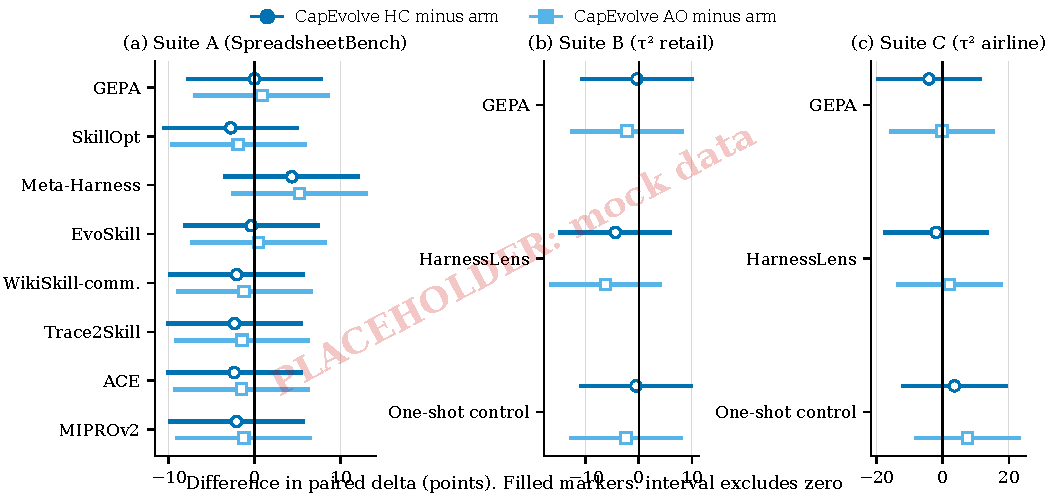
\includegraphics[width=\textwidth]{figures/fig_contrast.pdf}
\caption{Each \capevolve{} configuration against each competitor: an interval that excludes zero is a difference between the two, and one that spans zero is inconclusive. Differences are paired deltas in points with 95\% intervals (placeholder).}
\label{fig:contrast}
\end{figure*}

\begin{figure}[t]
\centering
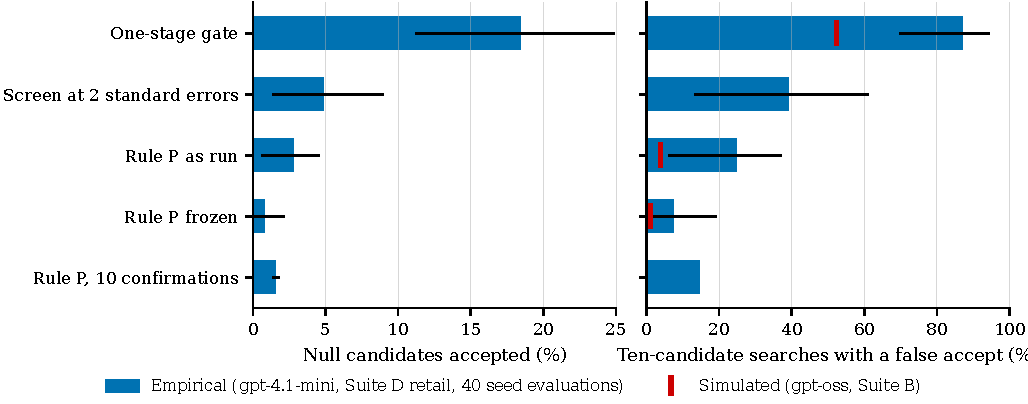
\includegraphics[width=\columnwidth]{figures/fig_nullpool.pdf}
\caption{On repeated evaluations of the unmodified seed, each gate promotes falsely in the share of searches shown, against the simulated value in red (placeholder).}
\label{fig:nullpool}
\end{figure}
